%%%%%%%%%%%%%%%%%%%%
%  DOCUMENT CLASS  %
%%%%%%%%%%%%%%%%%%%%

\documentclass[hyphens,twocolumn,nobalancelastpage,aps,10pt,citeautoscript,longbibliography]{revtex4-2}

%%%%%%%%%%%%%%
%  PACKAGES  %
%%%%%%%%%%%%%%
\nonstopmode%
\usepackage{url}
\usepackage[table,xcdraw,svgnames]{xcolor}
\usepackage{listings,engord,graphicx,bm,siunitx,xfrac,newpxtext}
\usepackage{natbib}
\usepackage[colorlinks]{hyperref}
\hypersetup{
	colorlinks=true,
	citecolor=black,
	linkcolor=DimGrey,
	urlcolor=DimGrey,
	breaklinks=true
}
\usepackage[english]{babel}
\usepackage[T1]{fontenc}
\usepackage[version=4]{mhchem}
\usepackage[a4paper, portrait, margin=2.54cm]{geometry}
\usepackage[compact]{titlesec}
\usepackage{color}
\definecolor{deepblue}{rgb}{0,0,0.5}
\definecolor{deepred}{rgb}{0.6,0,0}
\definecolor{deepgreen}{rgb}{0,0.5,0}

%%%%%%%%%%%%%%
%  SETTINGS  %
%%%%%%%%%%%%%%

\graphicspath{ {./images/} }

\setlength{\parskip}{1em} \lstdefinestyle{mystyle}{
	commentstyle=\color{deepgreen}, keywordstyle=\color{deepred},
	stringstyle=\color{codeblue}, basicstyle=\ttfamily,
	breakatwhitespace=false, breaklines=true,
	emphstyle=\ttb\color{deepred}, captionpos=b, keepspaces=true,
	numbers=left, numbersep=5pt, showspaces=false,
	showstringspaces=false, showtabs=false, tabsize=2 }
\lstset{style=mystyle}

\newcommand{\cay}[1]{\citeauthor{#1} (\citeyear{#1})~\cite{#1}}
\newcommand{\rhob}[0]{\rho_\textrm{bulk}}
\newcommand{\density}[0]{\kilogram\per\metre\cubed}

%%%%%%%%%%%%%%%%%%%%%%
%  DOCUMENT CONTENT  %
%%%%%%%%%%%%%%%%%%%%%%

\begin{document}

\title{Technical report: Exercise 2}

\author{Nhat Pham}

\begin{abstract}
	For Problem 1, using Euler method for solving ODEs, it is found that
	according to the simulation, Baumgartner did break the sound barrier with a
	fall of duration \qty{277}{\second} and a maximum speed which reached
	\qty{348}{\metre\per\second}. For Problem 2, a Gaussian wavepacket was
	successfully simulated using the finite differences method to solve PDEs
	(in this case the wave equation) for $\gamma = 1$, and investigating
	$\gamma \neq 1$ shows unstable regions for $\gamma > 1$, while for $\gamma
	< 1$, the models exhibit wave behaviour but far from the accuracy of the
	model when $\gamma = 1$.
\end{abstract}

\maketitle

\section{PROBLEM 1: FREEFALL WITH DRAG}%
\label{sec:problem_1}

\subsection{Introduction}%
\label{sub:introduction_1}

\noindent Problem 1 required solving ordinary differential equations (ODE) in
the form of Newtonian equations of motion. These are second order ODEs.\ The
situation is of Felix Baumgartner free-falling from a great height $y_0$, with
air resistances taken into account. Some parameters were given an appropriate
value or range of values, some had to be estimated. The drag coefficient of
Baumgartner was set to 1.0, the cross sectional area \qty{0.4}{\metre\squared},
and the mass \qty{70}{\kilogram}.

Part (a) called for a simple evaluation of the position and speed of the person
free-falling analytically. Part (b) called for the Euler method, which requires
two first order equations to solve the second order Newtonian ODE.\ Part (c)
asks to vary the air density, which was a constant $\rho_0$ in previous parts.
Part (d) used the free-fall results from part (c), but required an additional
calculation---the speed of sound, to examine whether or not Baumgartner would
break the sound barrier.

\subsection{Theory}%
\label{sub:theory_1}

\noindent The Euler method involves a set of iterations which only requires the
initial position and speed, $y_0$ and \qty{0}{\metre} respectively, a timestep
$\delta t$ is also defined, which separates each iteration (see
Equations~\ref{eq:velocity},~\ref{eq:position}, and~\ref{eq:time})
\begin{equation}
	\label{eq:velocity}%
	v_{y,n+1} = v_{y,n} - \delta t \left(g + \frac{k}{m}|v_{y,n}| v_{y,n}\right)
\end{equation}
\begin{equation}
	\label{eq:position}%
	y_{n+1} = y_n + \delta t \cdot v_{y,n}
\end{equation}
\begin{equation}
	\label{eq:time}%
	t_{n+1} = t_n + \delta t
\end{equation}

\subsection{Method}%
\label{sub:method_1}

\noindent Part (a) was straightforward since the analytical equations were
given and evaluation required only an array of time.

For part (b), To calculate $y_{n+1}$ requires $\delta t$, $y_{n}$ and also
$v_{n}$. This means the order of which values were filled would be $t$, $v$ and
then $y$. This all happens within a \lstinline{for} loop, and vectorisation did
not seem plausible since the current indexed value is calculated using the
previous indexed value. To examine the effect on varying the timestep $\delta
	t$, the simulation was repeated for several timesteps between
0.1--\qty{7}{\second} and to quantify the error, the standard deviation of the
difference $\delta y$ between the analytical trajectory and the numerical
trajectory was calculated. A similar method was used for vertical speed. To
examine the effect of the quantity $k/m$ on the motion, the mass $m$ is varied
between 50--\qty{80}{\kilogram} and $k$ here is kept constant.

For part (c), the drag factor $k$ now becomes a function of $y$, $k(y)$. The
consequence of this is that whereas before $v_{n+1}$ did not depend on $y$, but
since it depends on $k$, which is now a function of $y$, it also depends on
$y$. The same method for part (b) is used, but now the drag factor has to also
be calculated at each step, since the altitude changes every step.

For part (d), because the speed of sound $v_s$ is a function of temperature
$T$, and $T$ is a function of $y$, $v_s$ is a function of $y$, $v_s(y)$. Since
the simulation is discrete, the speed of sound is calculated using the $y$
values obtained from part (c). The Mach ratio is then calculated, which is the
ratio $v/v_s$.

To test what affects the Mach number, jump height and drag coefficient was
varied between 1000--\qty{40000}{\metre} and 0.05--2.0 respectively, keeping
all other quantities the same (using Baumgartner's scenario).

\subsection{Results and discussions}%
\label{sub:results_and_discussions_1}

\noindent For part (a), two plots were generated, one for
position and one for speed (Figure~\ref{fig:freefall_analytic}). Additionally,
the result arrays were trimmed when the body reaches the ground.
\begin{figure*}[htpb]
	\centering
	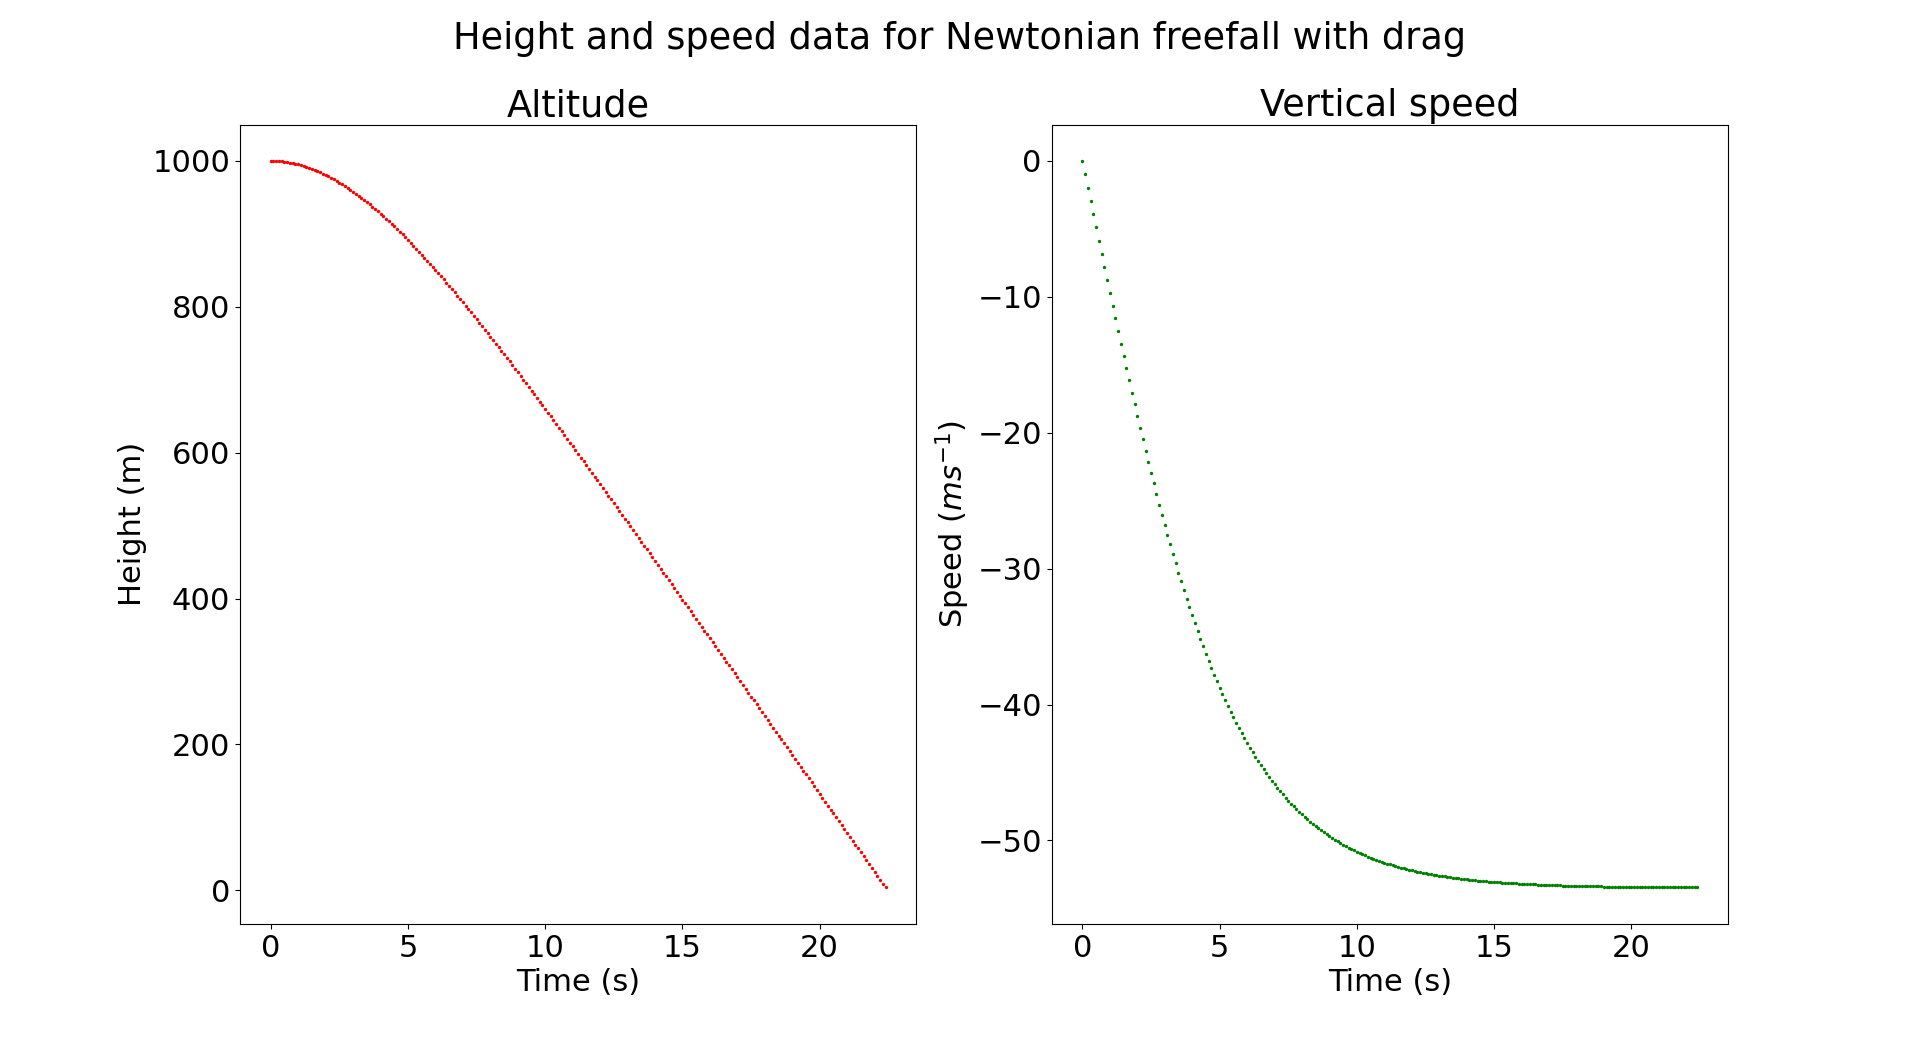
\includegraphics[width=\linewidth]{freefall_analytic.png}
	\caption{Analytical predictions of a free-falling body.}%
	\label{fig:freefall_analytic}
\end{figure*}

For part (b), two plots were generated, one for position and one for speed
(see Figure~\ref{fig:freefall_numeric}). The numerical prediction got close to
the actual trajectory, which is the analytical prediction. The body stopped at
similar times (part (a) predicts $t_f = \qty{22.468}{\second}$ while part (b)
predicts $t_f = \qty{22.400}{\second}$).
\begin{figure*}[htpb]
	\centering
	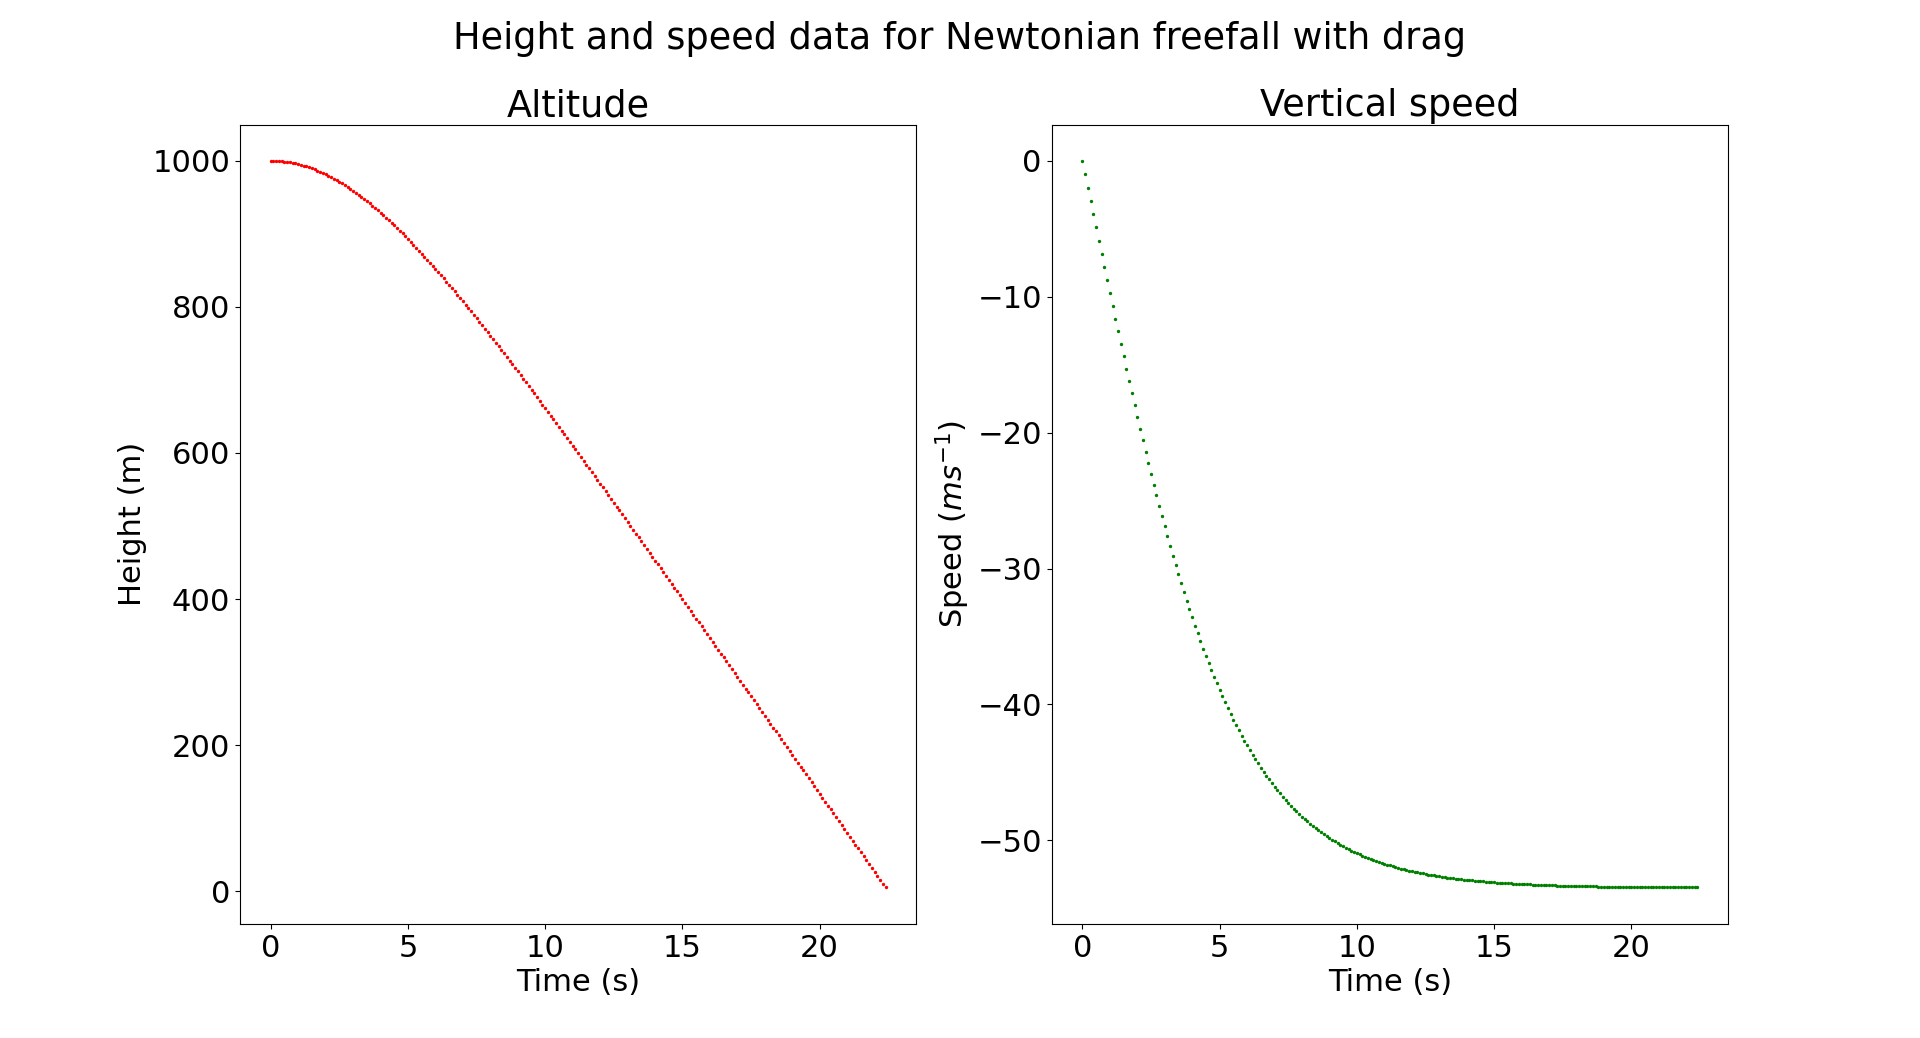
\includegraphics[width=\linewidth]{freefall_numeric.png}
	\caption{Numerical predictions of a free-falling body using Euler method.}%
	\label{fig:freefall_numeric}
\end{figure*}

On examining the effect of varying timestep, two plots were generated (see
Figure~\ref{fig:timestep_std}). From both plots, it can be said that an
increase in timestep increases the standard deviation in both position and
speed. More interestingly, discontinuous features are seen in both plots, which
makes the plots look like they consist of linear regions of different gradients
stitched together, but with discontinuous jumps. The position plot (left)
overall seems to be a quadratic increase in error. The speed plot (right)
starts off appearing slightly quadratic but mostly linear, followed by a region
where there exhibits no correlation (i.e.\ constant horizontal), this region is
small and occurs roughly around $\delta t = \qty{5}{\second}$. After that,
there is rapid increase similar to the position plot.
\begin{figure*}[htpb]
	\centering
	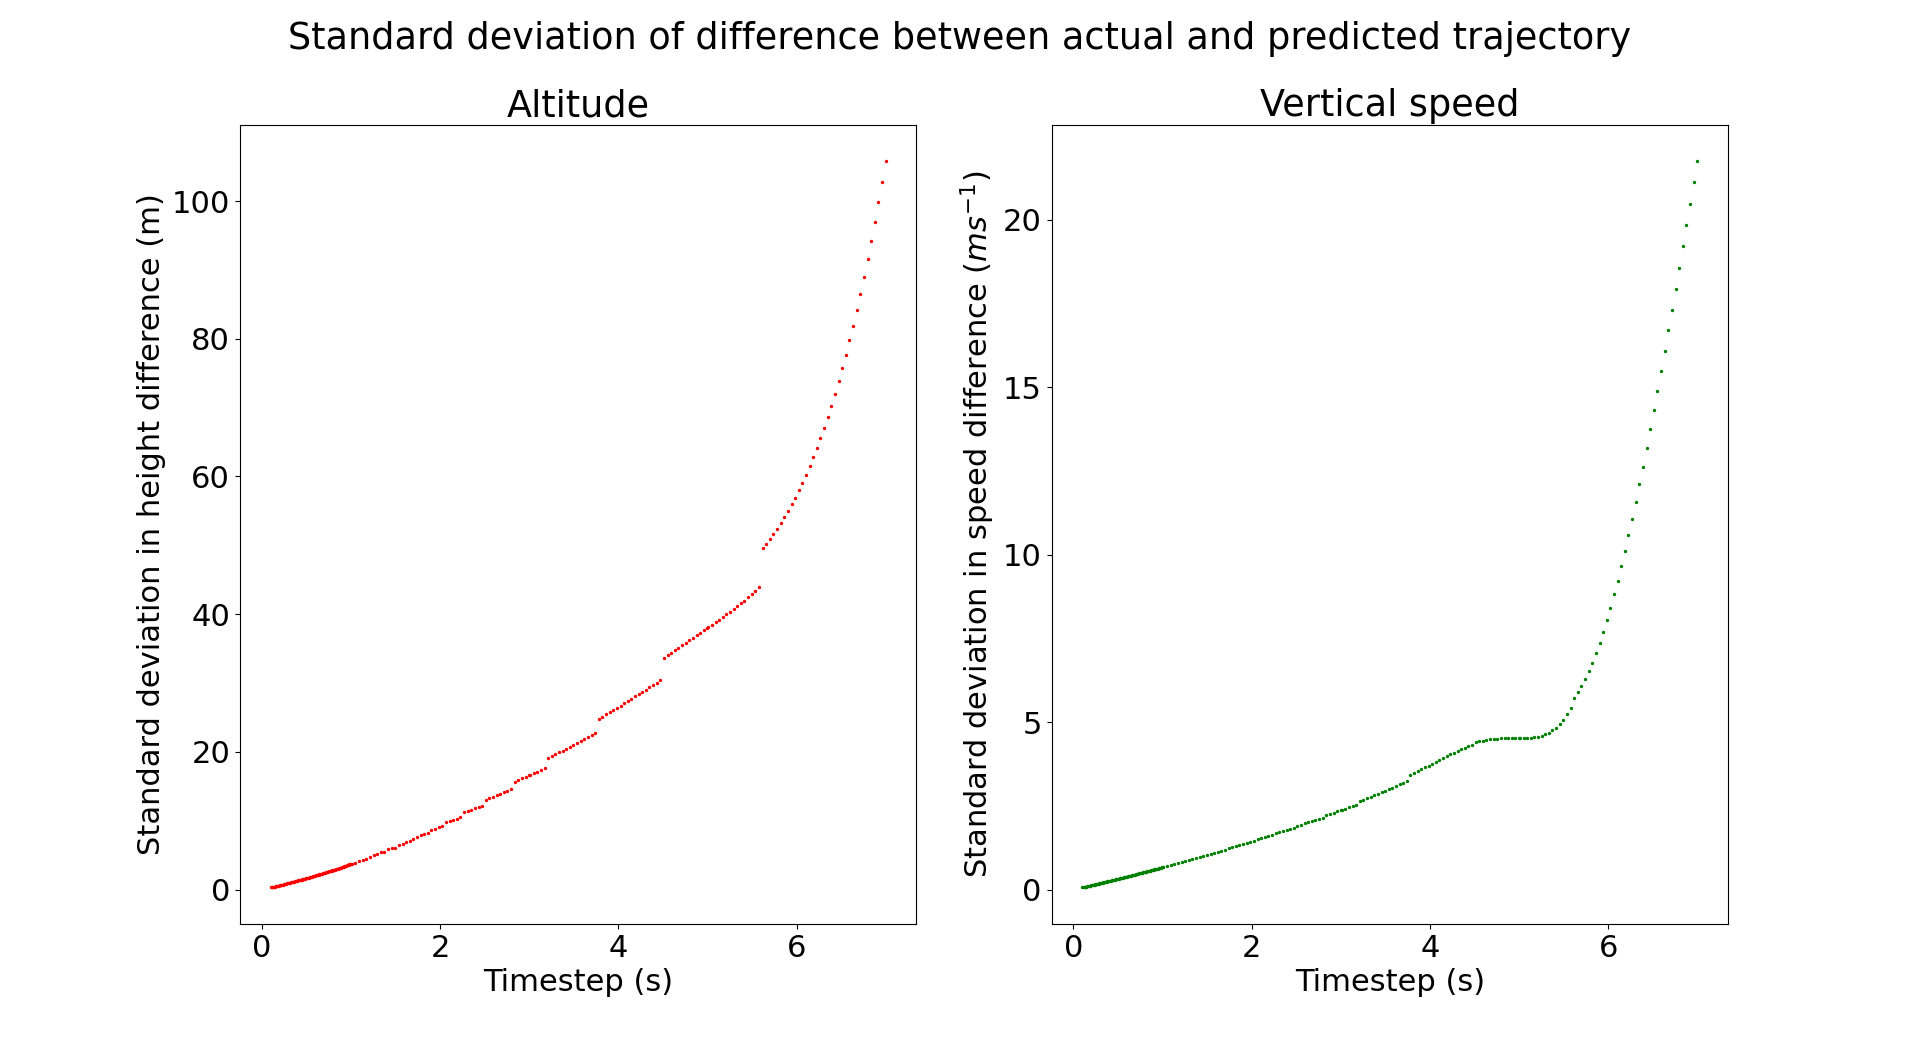
\includegraphics[width=\linewidth]{timestep_std.png}
	\caption{Investigating the effect of simulation timestep $\delta t$ on the accuracy of the simulation}%
	\label{fig:timestep_std}
\end{figure*}

On examining the effect of varying $k/m$, the duration of the fall and the
maximum speed achieved during the fall was plotted as a function of mass (see
Figure~\ref{fig:mass_duration_speed}). A larger mass seems to shorten fall
duration, with a change that appears to be almost linear or slightly quadratic.
A larger mass also increases the maximum speed at the order of $\sim 10^1$
\qty{}{\metre\per\second} for the range of mass used, with a change that also
appears to be almost linear or slightly quadratic.
\begin{figure*}[htpb]
	\centering
	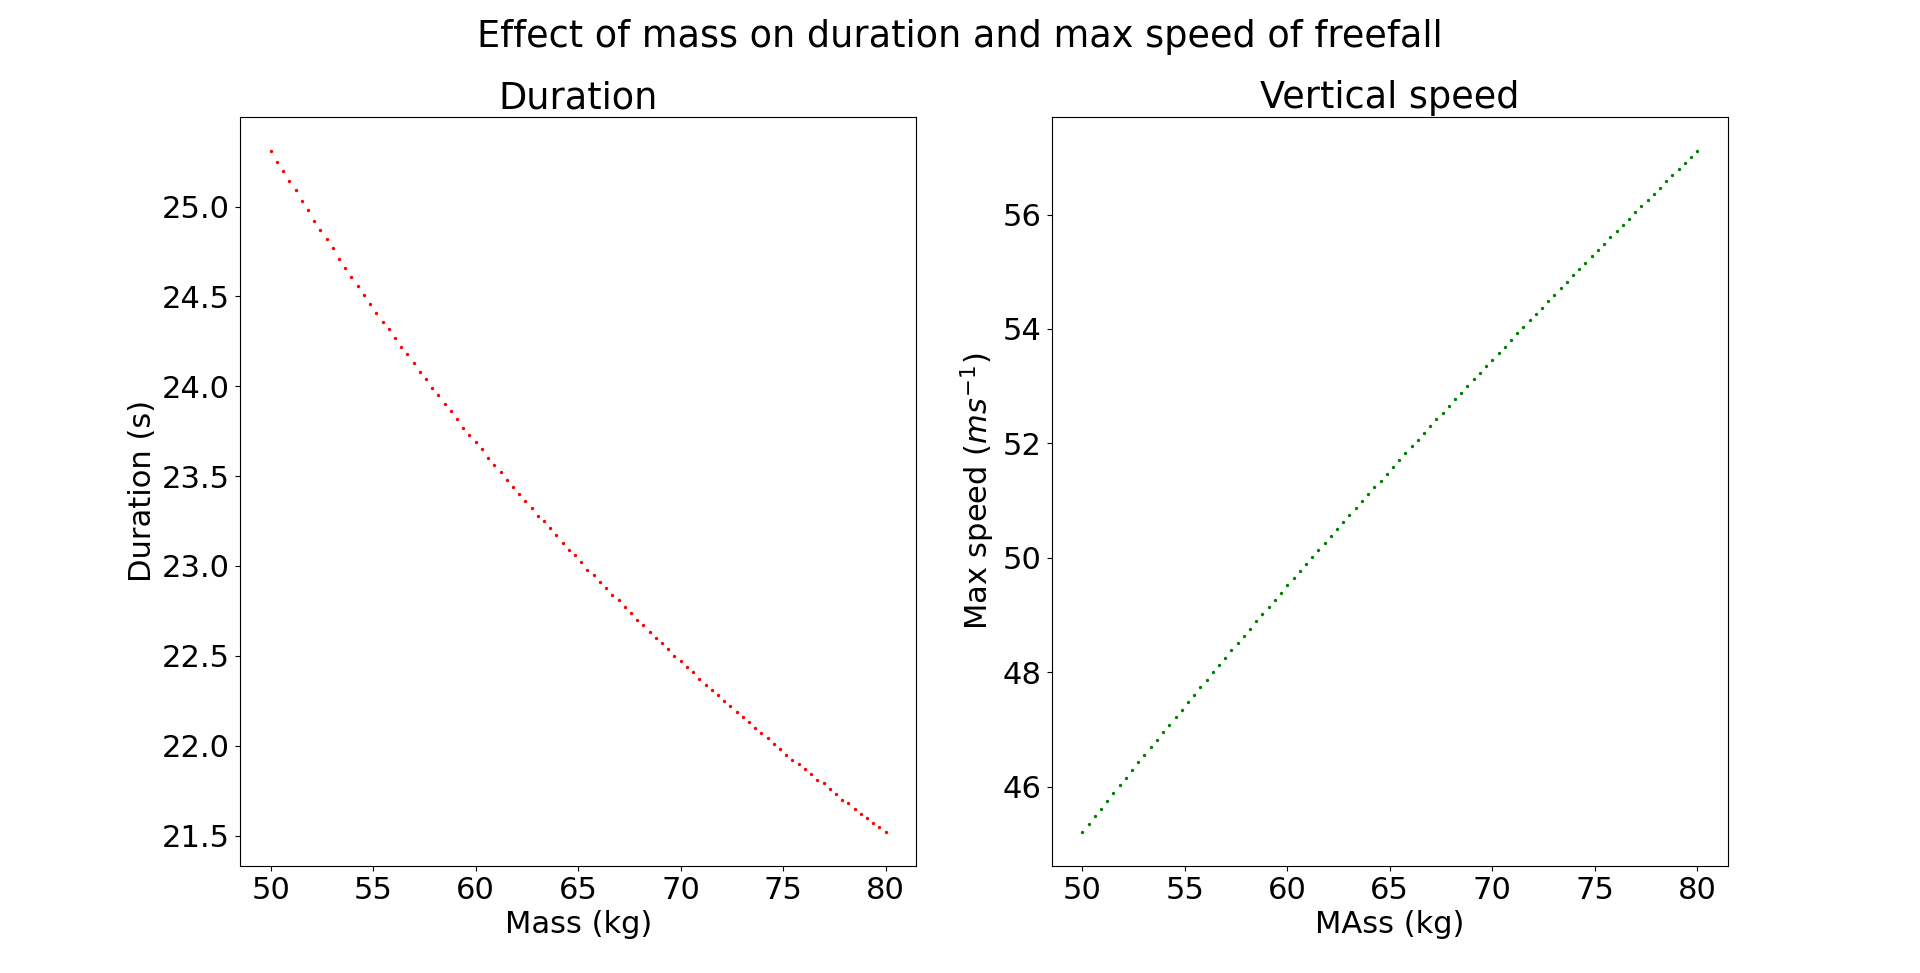
\includegraphics[width=\linewidth]{mass_duration_speed.png}
	\caption{Investigating the effect of mass $m$ of the body on duration and maximum speed of a freefall}%
	\label{fig:mass_duration_speed}
\end{figure*}

For part (c), the value $y_0 = \qty{39045}{\metre}$ was used here to match
Baumgartner's initial conditions. Similar to (a) and (b), two plots were
generated for position and speed
(Figure~\ref{fig:freefall_numeric_varying_air_density}). A minimum is observed
in the speed versus time plot, which indicates that the body reaches a downward
speed much higher than the terminal velocity. For reference, if the body were
to fall without varying air density, its trajectory, with Baumgartner's initial
conditions would look like Figure~\ref{fig:freefall_numerical_big}. The body
would have taken more than twice as long to reach the ground, and its speed
does not surpass the terminal velocity of $v \approx
	\qty{55}{\metre\per\second}$. On the other hand, if the air density varies,
then the downward speed reaches a magnitude of $\sim 10^2$. By varying the air
density, the simulation is more realistic as it produces values closer to what
actually happened.
\begin{figure*}[htpb]
	\centering
	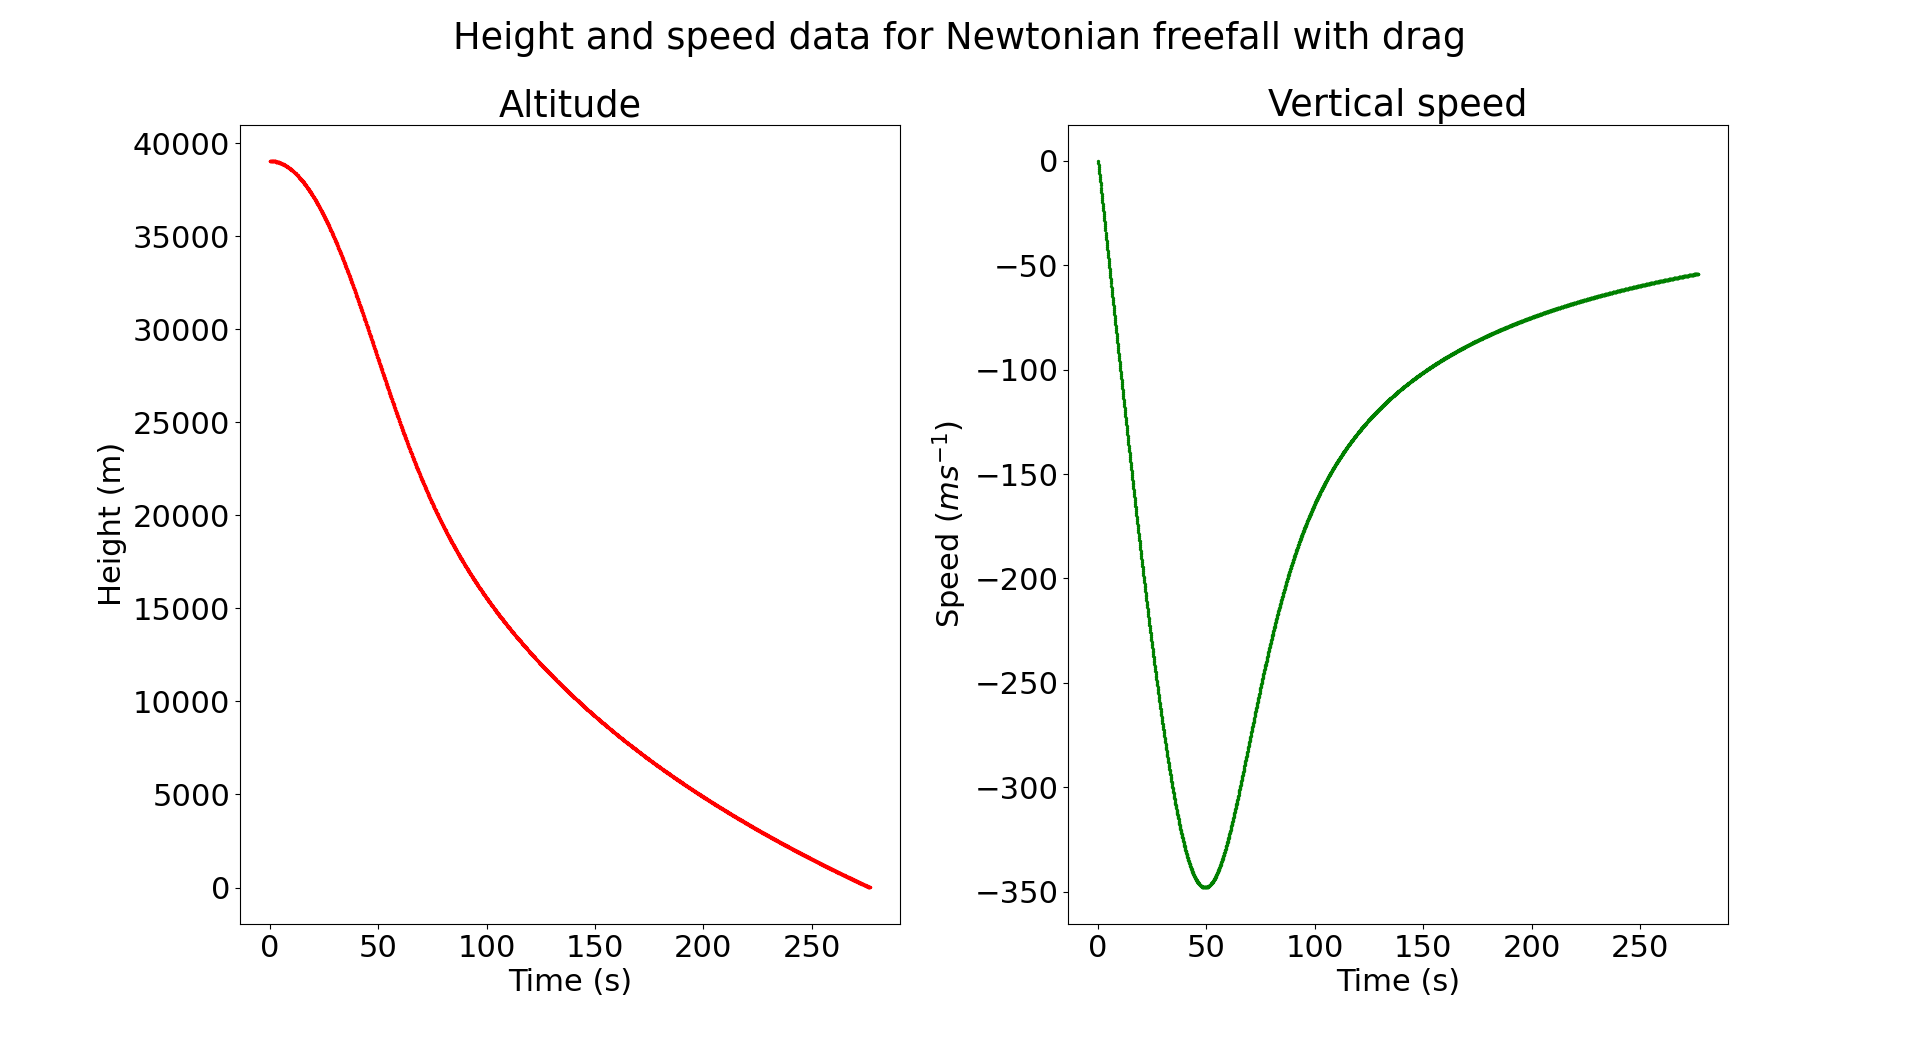
\includegraphics[width=\linewidth]{freefall_numerical_varying_air_density.png}
	\caption{Numerical predictions of a free-falling body using Euler method, with air density varying as a function of position. Using Baumgartner's initial height}%
	\label{fig:freefall_numeric_varying_air_density}
\end{figure*}
\begin{figure*}[htpb]
	\centering
	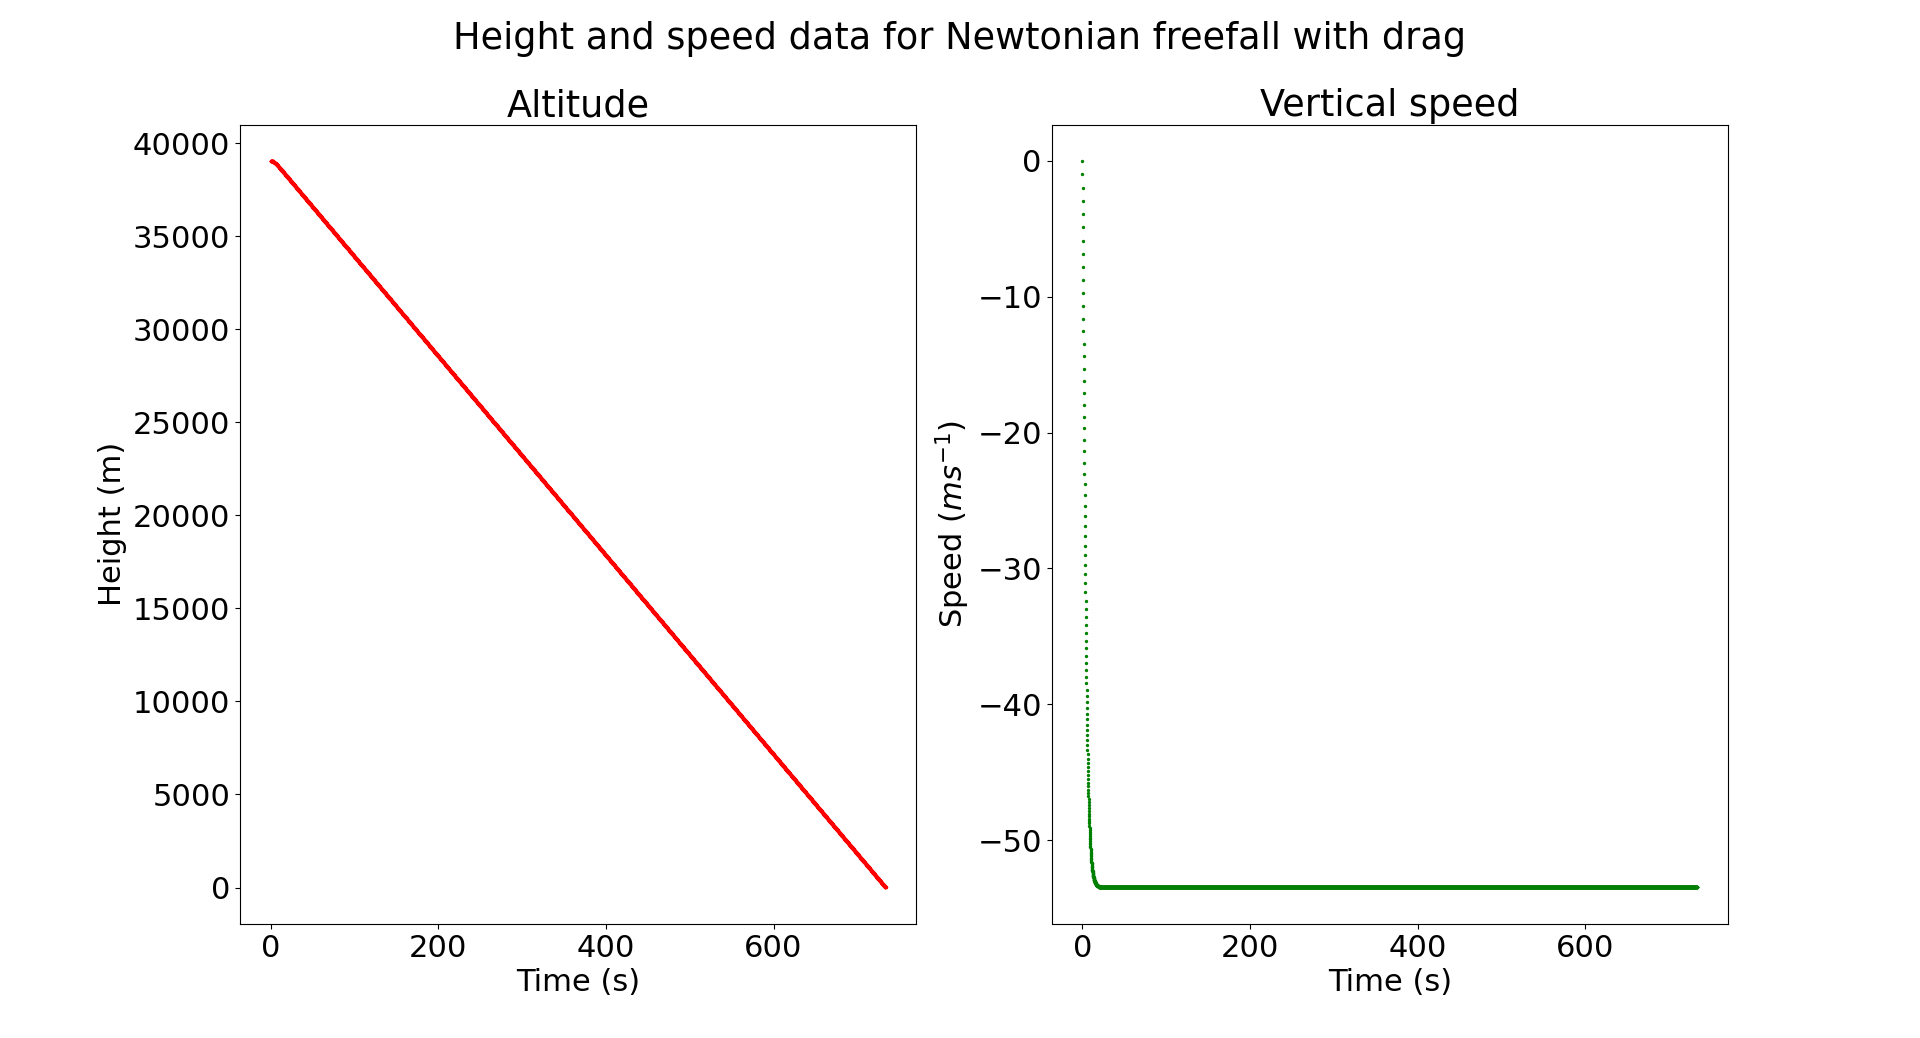
\includegraphics[width=\linewidth]{freefall_numerical_big.png}
	\caption{Numerical predictions of a free-falling body using Euler method. Using Baumgartner's initial height}%
	\label{fig:freefall_numerical_big}
\end{figure*}

For part (d), Baumgartner's fall reaches the maximum Mach number is 1.180 (to 3
d.p.), while the maximum speed is \qty{348.030}{\metre\per\second} (to 3 d.p.).
The plot for this is shown in Figure~\ref{fig:mach_ratio}. There is a spike in
the Mach ratio at around \qty{50}{\second}, which seems correct since
in~\ref{fig:freefall_numeric_varying_air_density}, there is a spike in
downwards speed at the same time. It appears that he would have broken the
sound barrier, and this behaviour can be explained by the varying air density
at different altitudes---without accounting for this, the jumper cannot reach a
speed that great.
\begin{figure*}[htpb]
	\centering
	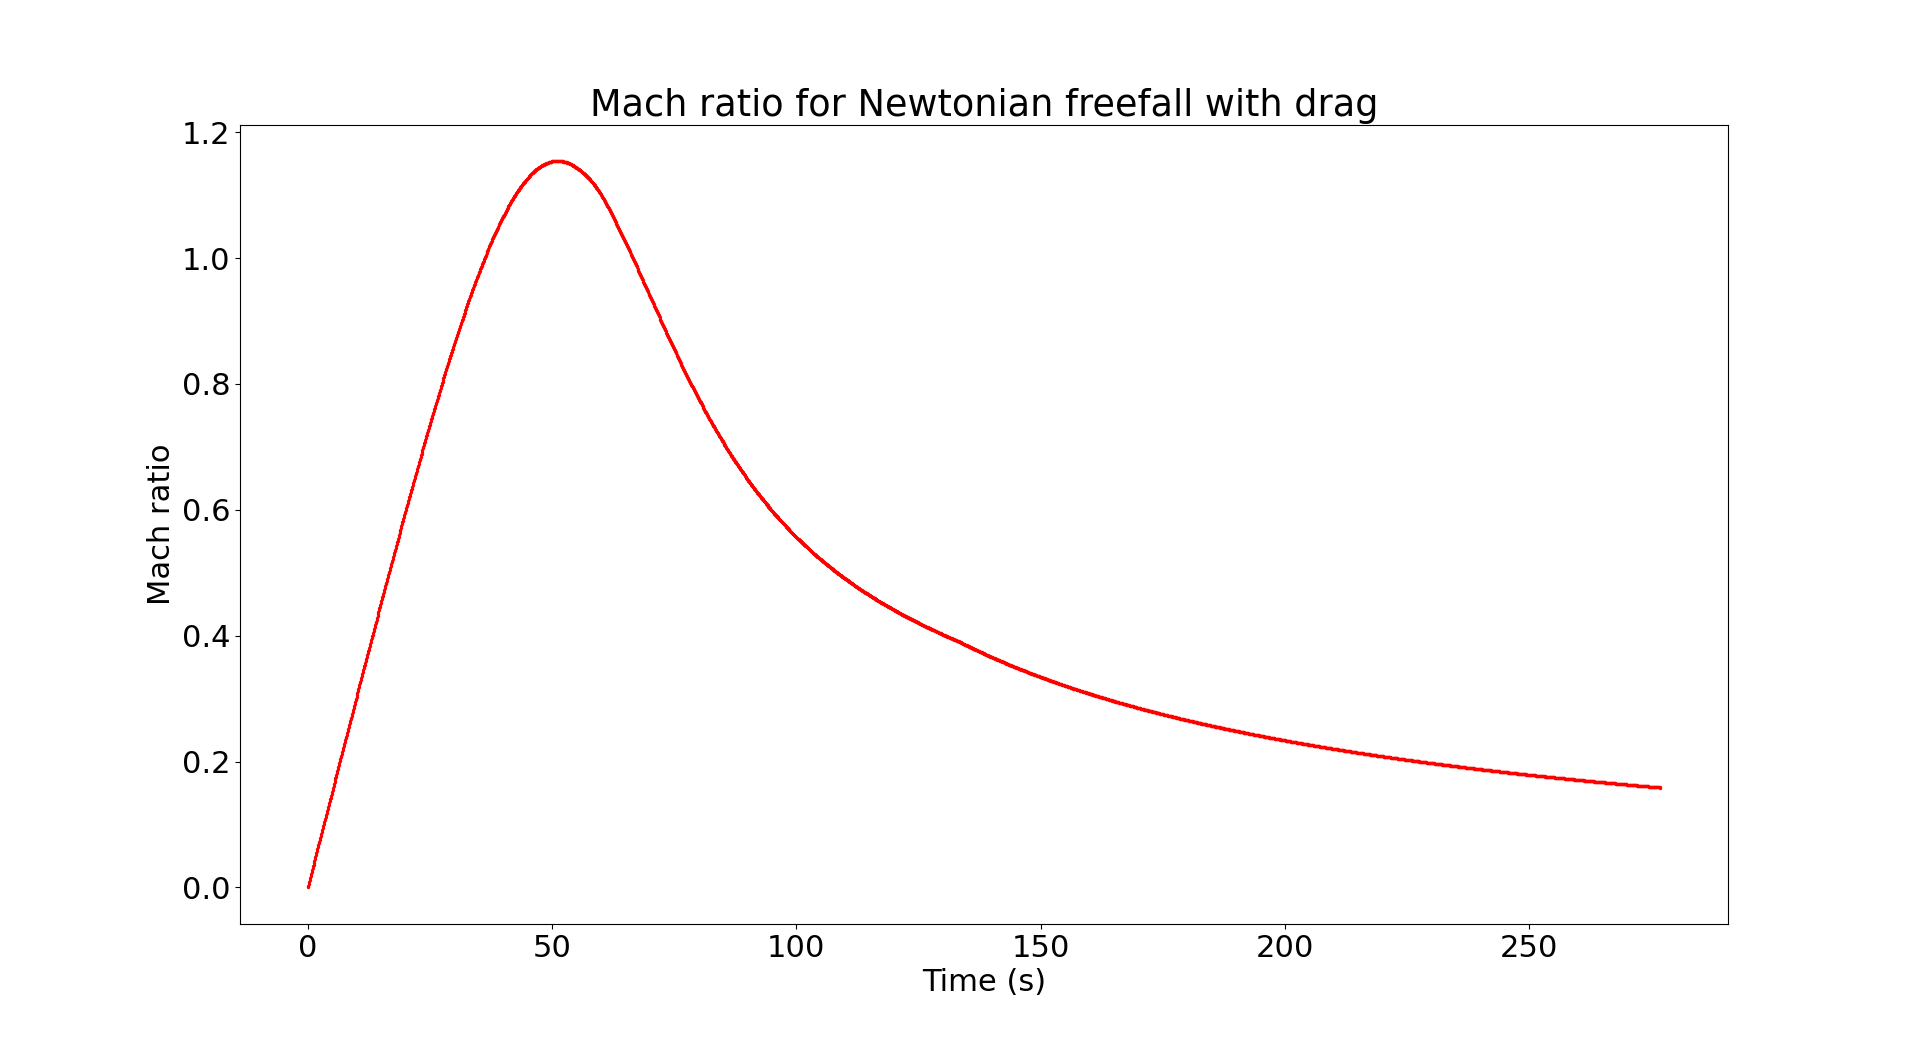
\includegraphics[width=1\linewidth]{mach_ratio.png}
	\caption{The ratio between Baumgartner's downwards speed and the speed of sound}%
	\label{fig:mach_ratio}
\end{figure*}

Three plots were generated for the maximum Mach number achieved (red), the maximum
speed (green), and also the duration of the fall (blue). The Mach number
increases with height, and appears to break the sound barrier (when it's larger
than 1) above \qty{30000}{\metre}. This correlation appears to be linear for
the most part, but at the start there is a lesser increase. The duration plot
shows that increasing the height increases the duration logarithmically.
\begin{figure*}[htpb]
	\centering
	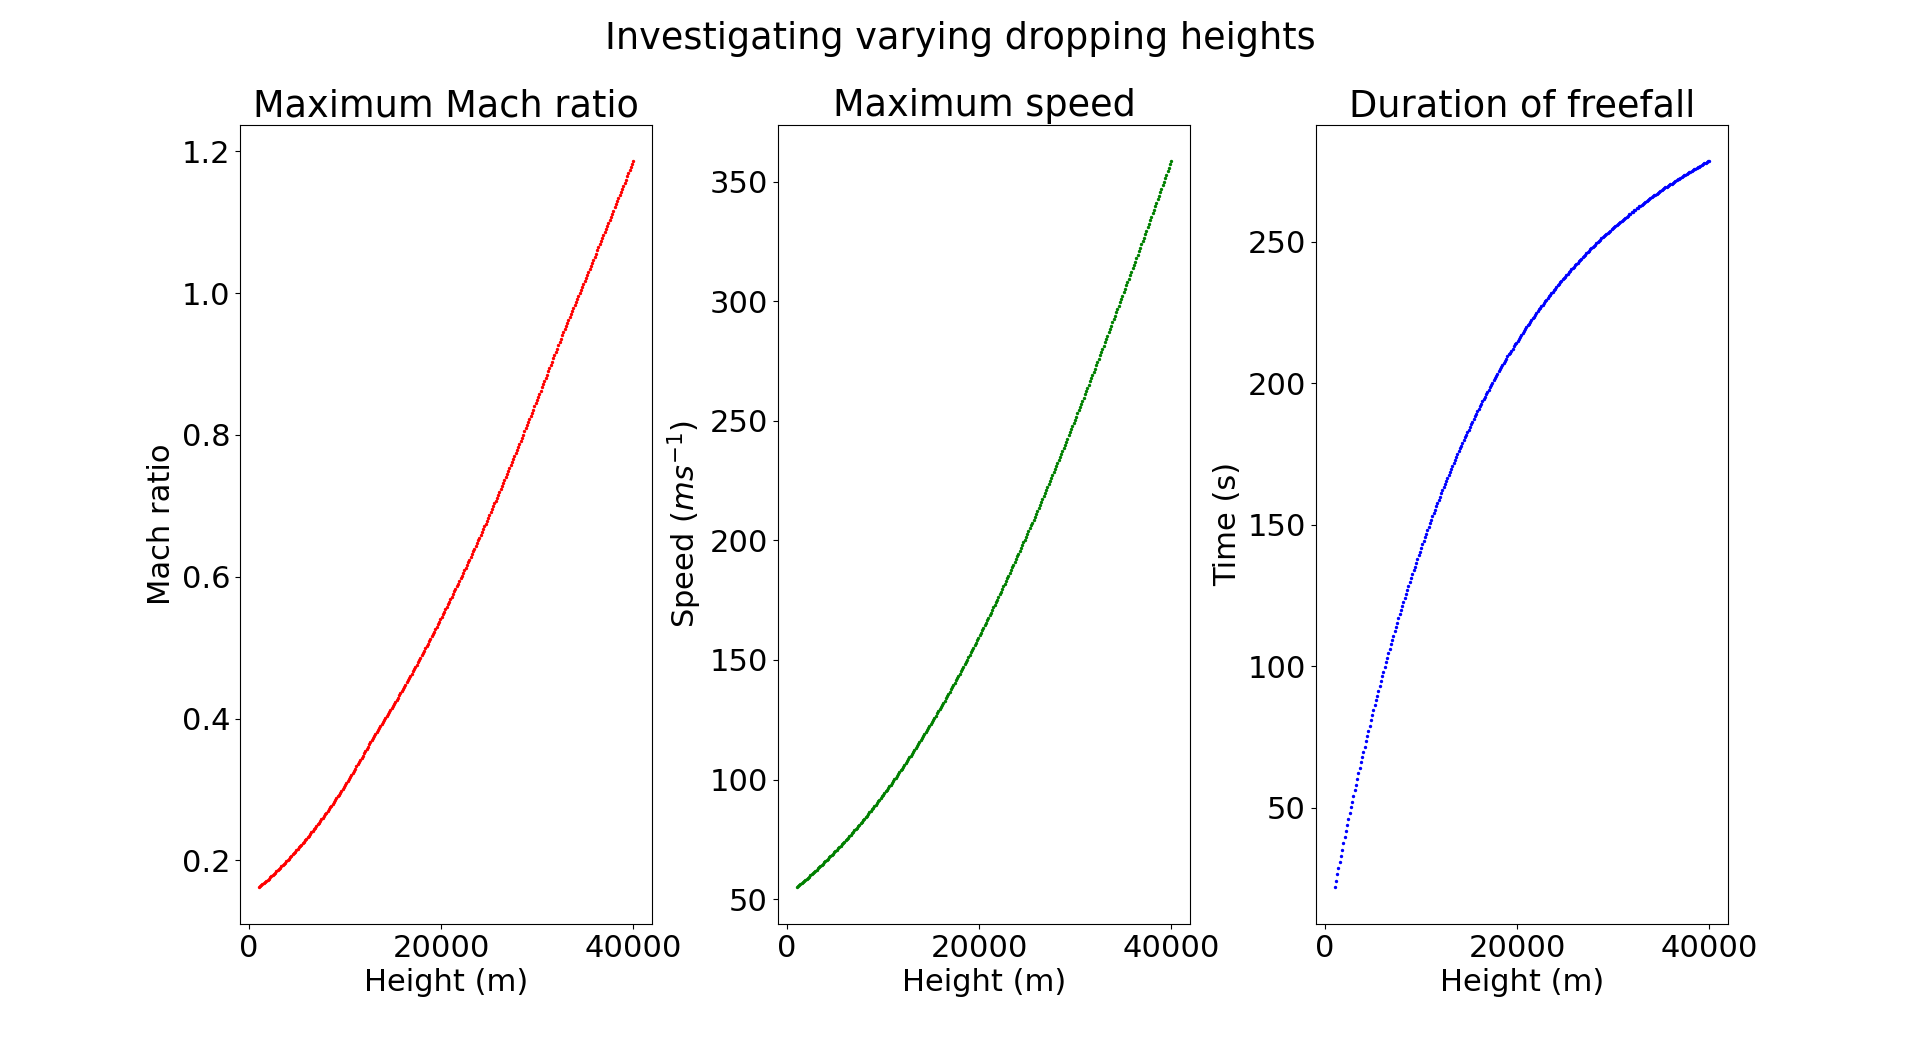
\includegraphics[width=\linewidth]{jump_height.png}
	\caption{Investigating the effect of jump height $y_0$ on the maximum speed achieved during freefall}%
	\label{fig:jump_height}
\end{figure*}

For jump height, three plots were likewise generated. As expected, increase the
drag coefficient makes the falling object less aerodynamics, which results in a
lower maximum speed achieved (middle green plot from
Figure~\ref{fig:drag_coeffs}). However, it appears that the sound barrier can
be breached even with a drag coefficient of $\sim$ 1.75. The decrease in Mach
ratio as drag coefficient increases appears to be exponential, while the
duration increases logarithmically.
\begin{figure*}[htpb]
	\centering
	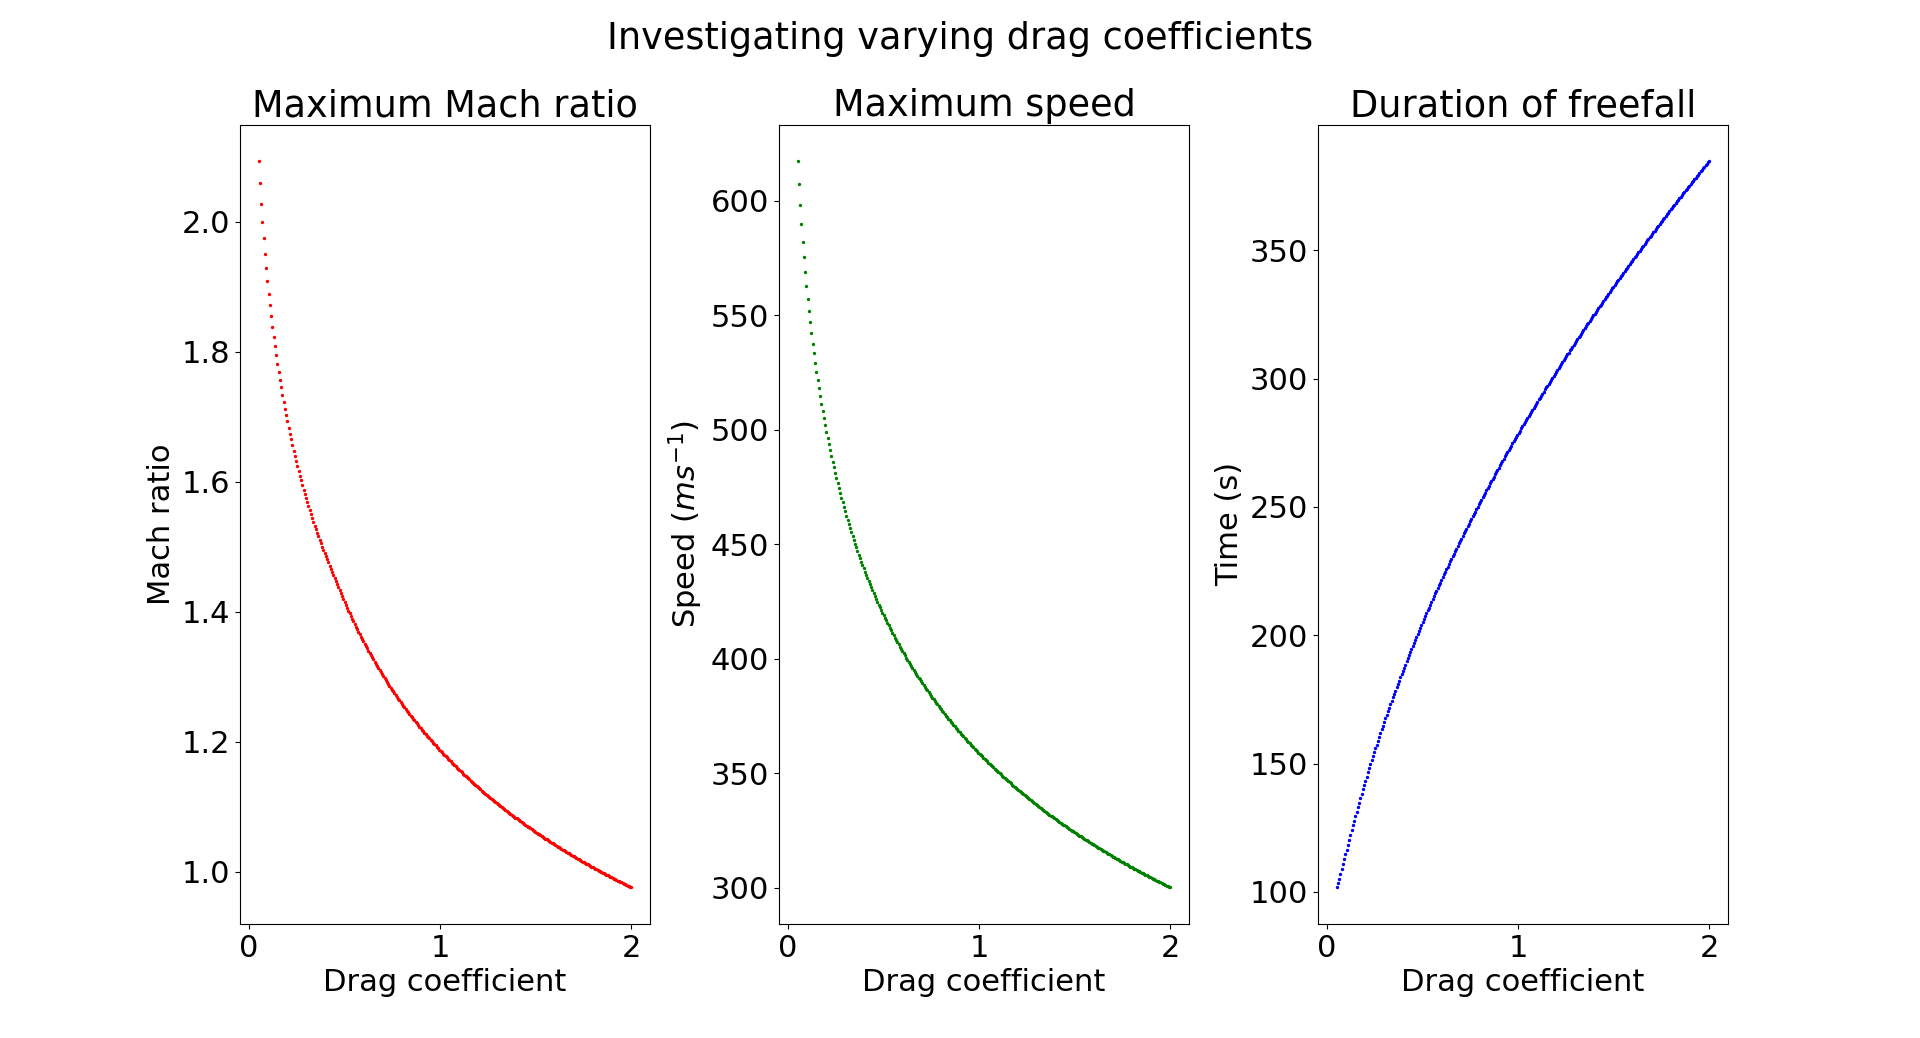
\includegraphics[width=\linewidth]{drag_coeffs.png}
	\caption{Investigating the effect of drag coefficient $C_d$ on the maximum speed achieved during freefall}%
	\label{fig:drag_coeffs}
\end{figure*}

Overall, a timestep $\delta t$ was chosen so that the standard deviation from
the actual solution was small ($\delta t = \qty{0.1}{\second}$). Nevertheless,
the final values were not exactly identical to values from the actual freefall.
Baumgartner in reality fell for \qty{259}{\second} with maximum speed
\qty{373}{\metre\per\second} while in the simulation he was airborne for
\qty{277}{\second} and reached \qty{348}{\metre\per\second} (both values to 3
significant figures). The speed differed by a magnitude of $\sim
10^1\qty{}{\metre\per\second}$, or 6\% of the actual measured speed. Thus, the
accuracy in the result of part (c) or (d) (i.e.
Figure~\ref{fig:freefall_numeric_varying_air_density} and~\ref{fig:mach_ratio})
can be improved. If local truncation error was not small (in this case it was
small), then the modified Euler method could have been considered. This
requires an additional averaging of the slope from the original Euler method
with the slope of the starting point to give a more accurate derivative.
Nevertheless, improvements could be made by considering more physical factors
beyond varying air density. In reality, how air turbulence works can be
complicated and the motion of a body through air molecules can result in
physics which might lead to slightly different results. For example,
Baumgartner was tumbling around during his fall, so an average surface area was
taken, but if an estimation of surface area for every step was used (as he was
either falling down head first, or body first), this combined with varying air
density would yield a more accurate model.

\subsection{Conclusion}%
\label{sub:conclusion_1}

\noindent Baumgartner did break the sound barrier according to the simulation,
and the model and physical phenomena factored in did provide somewhat accurate
results (with a maximum speed within 6\% of actual maximum speed).

\section{PROBLEM 2: WAVE EQUATION}%
\label{sec:problem_2_wave_equation}

\subsection{Introduction}%
\label{sub:introduction_2}

\noindent Problem 2 required modelling a Gaussian wave on a string, which here
spans in the $x$ direction. The position of the wave in the $y$ direction at
any given time $t$ obeys the wave equation. Part (e) requires evaluating the
solution of the partial differential equation (PDE), $u(x,t)$ numerically, and
the finite differences method is used. Part (f) examines the effects of the
model from part (e) for different values of $\gamma$.

\subsection{Theory}%
\label{sub:theory_2}

\noindent The finite differences method was used to solve the wave equation for
a 1-dimensional string (in the $x$ direction) (Equation~\ref{eq:finite_differences})
\begin{equation}
	\begin{aligned}
		u(x,t+\tau) =\,\, & \gamma[u(x+q,t)                 \\
		                  & + u(x-h,t)]                     \\
		                  & + 2u(x,t)(1-\gamma)-u(x,t-\tau)
	\end{aligned}
	\label{eq:finite_differences}%
\end{equation}
With the zeroth timestep $u(x,0)$ initialised by a Gaussian wavepacket, and the
first timestep $u(x,\delta t)$ calculated using the central difference method
(Equation~\ref{eq:central_difference}).
\begin{equation}
	\label{eq:central_difference}%
	\begin{aligned}
		u(x,\tau) =\,\, & \frac{1}{2}[u(x+h, 0)            \\
		                & u(x-h,0)] + \tau u^{\prime}(x,0)
	\end{aligned}
\end{equation}
\subsection{Method}%
\label{sub:method_2}

\noindent For part(e), the finite differences method requires two initial
timesteps, of which the first can be calculated using the Gaussian equation
given, and the second using the Gaussian equation and its derivative.
Sequential timesteps can then be computed using the finite differences formula.
At each timestep, the positions of all points are plotted and saved as an image
in the directory of the running program.

The calculation of the initial timesteps and the proceeding timesteps can all
be vectorised with numpy arrays. In this numerical solution, the value $\gamma
	\approx 1$ gives the exact solution of the wave equation, but by fixing
$\gamma$, this puts limits on the other properties of the wavepacket or the
string. Since the length density $\mu$ is kept constant, the tension $T$ in the
string has to be tuned so that the phase velocity ($v = \sqrt{T/\mu}$)
satisfies for $\gamma = 1$.

For part (f), the simulation from part (e) was repeated for values of gamma
from 0.1--1.32. To measure the difference in the actual solution versus the
model, the standard deviation of the difference between positions was computed
for each timestep, and then an average was computed for all timestep so that
each gamma value has a corresponding error value.

\subsection{Results and discussions}%
\label{sub:results_and_discussions_2}

\noindent For part (e), three timesteps of the wave is shown in Figure~\ref{fig:gamma_1}.
The wavepacket moves to the right, hits the right node and reflects back with
negative amplitude. These are all expected behaviours. The wave is seen to
return to its original starting point after around $t = \qty{6.10}{\second}$.
The wavepacket appears to have sensible motion that seems feasible. Its
amplitude becomes negative when reflected at the boundary $x=0$ and $x=L$, as
expected from a realistic system. A way of improving the simulation would be to
play around with values such as $A_0$ (the amplitude of the wave, which was
normalised in this case), Gaussian width $\sigma$ and even timestep $\delta t$
and investigate their effects on the simulation accuracy.
\begin{figure*}[htpb]
	\centering
	\includegraphics[width=\linewidth]{gamma-1.png}
	\caption{Wave propagation for a Gaussian wavepacket, $\gamma = 1$}%
	\label{fig:gamma_1}
\end{figure*}

For part (f), a plot was generated showcasing the error induced by varying
$\gamma$ (see Figure~\ref{fig:gamma_std}). Animations of waves for various
$\gamma$ were also generated and uploaded to the following link
(\url{https://imgur.com/a/zbUIvHW}) (along with $\gamma = 1$).
\begin{figure*}[htpb]
	\centering
	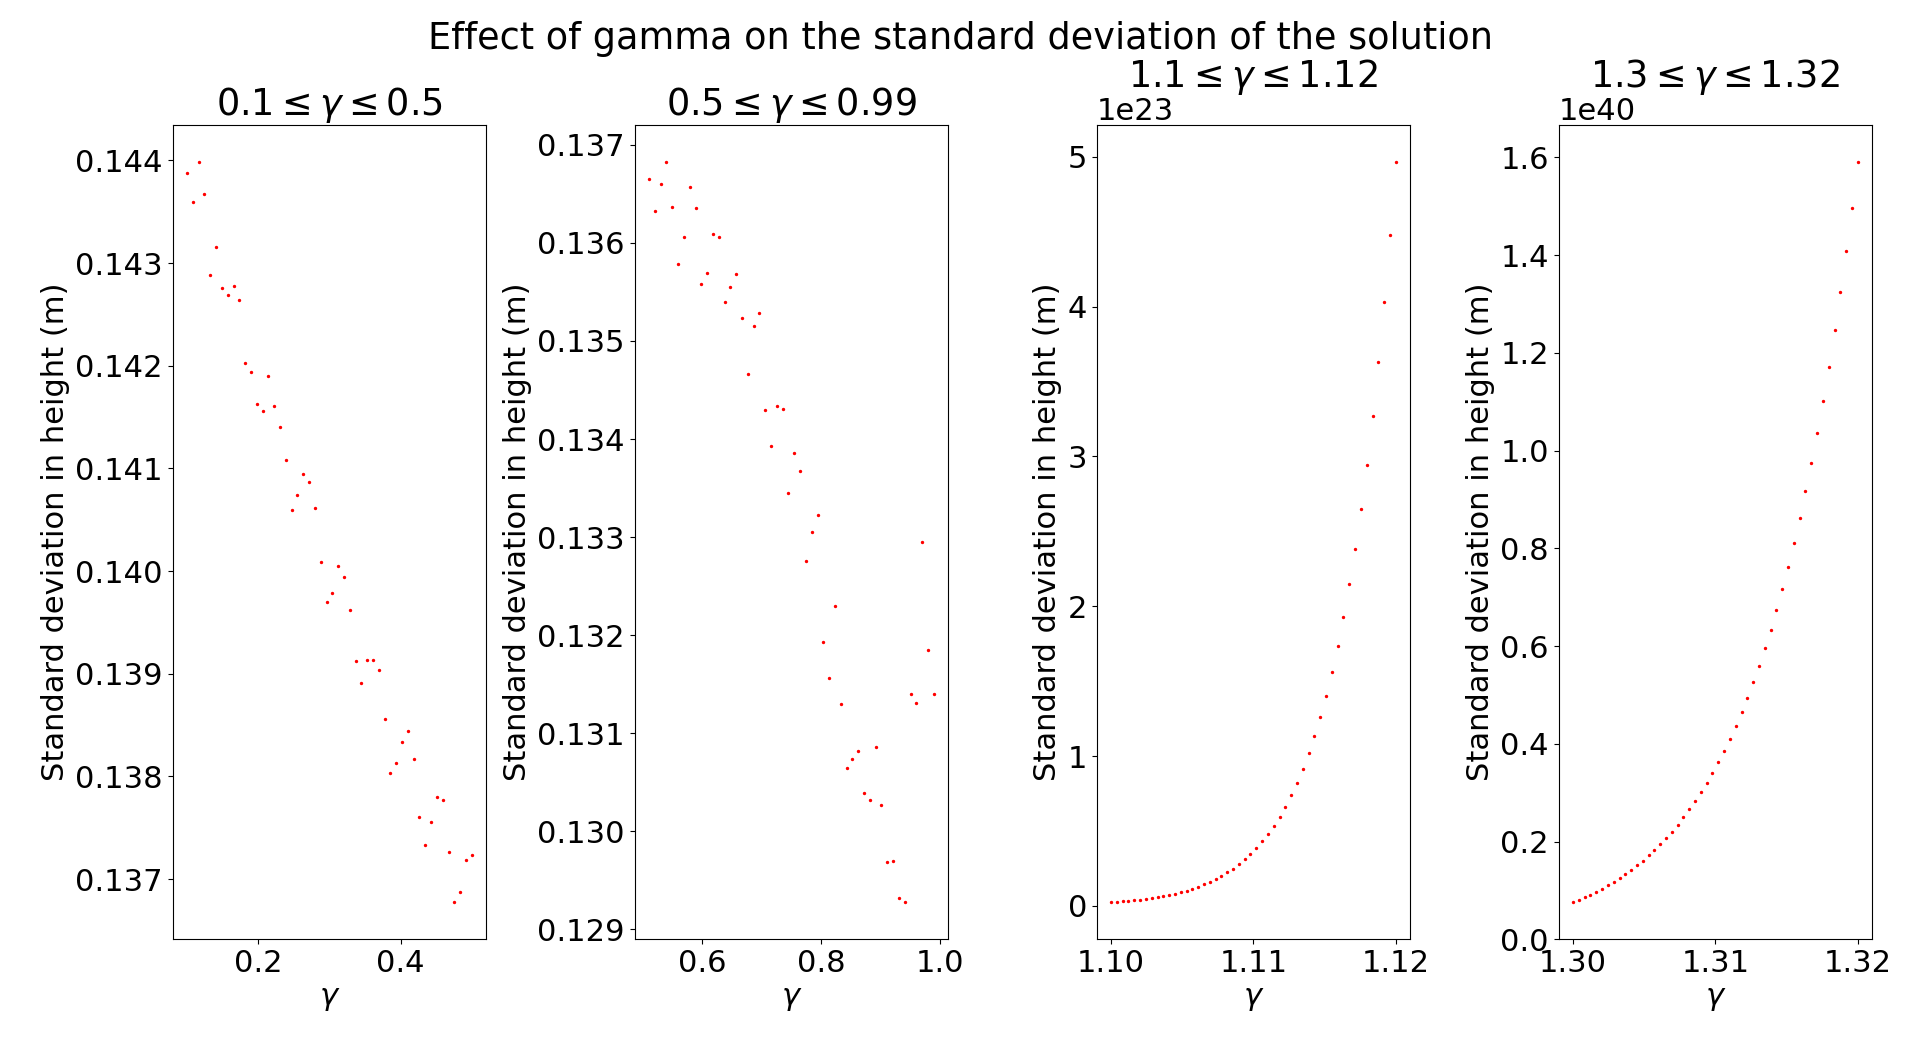
\includegraphics[width=\linewidth]{gamma_std.png}
	\caption{Effect of gamma on the standard deviation of the solution}%
	\label{fig:gamma_std}
\end{figure*}

It is seen that the standard deviation decreases linearly as $\gamma$
approaches $1$ on either side, except for the strange region around $\gamma
\approx 0.99$ where the standard deviation increases suddenly before becoming 0
at $\gamma = 1$ (see Figure~\ref{fig:gamma-0.99} for snapshots of $\gamma =
0.99$). This could happen possibly due to the simulation getting closer to the
actual solution, so that it has a phase velocity quite close to the actual
phase velocity, but since it deviates from the actual solution, but with more
``motion'', it can result to more deviation from the actual wave, as opposed to
lower values of $\gamma < 0.99$ because those seem to have a phase velocity
much lower (they are not moving to the right substantially, but staying almost
stationary and generating waves by oscillating transversely, see
Figure~\ref{fig:gamma-0.5} for phase velocity very close to
\qty{0}{\metre\per\second} and Figure~\ref{fig:gamma-0.88} for phase velocity
non-zero but not quite fast enough). For $\gamma$ below 1, it seems like the
increase in error is linear as $\gamma$ gets further from 1 and approaches $0$.
\begin{figure*}[htpb]
	\centering
	\includegraphics[width=\linewidth]{gamma-0.99.png}
	\caption{Wave propagation for a Gaussian wavepacket, $\gamma = 0.99$}%
	\label{fig:gamma-0.99}
\end{figure*}
\begin{figure*}[htpb]
	\centering
	\includegraphics[width=\linewidth]{gamma-0.5.png}
	\caption{Wave propagation for a Gaussian wavepacket, $\gamma = 0.5$}%
	\label{fig:gamma-0.5}
\end{figure*}
\begin{figure*}[htpb]
	\centering
	\includegraphics[width=\linewidth]{gamma-0.88.png}
	\caption{Wave propagation for a Gaussian wavepacket, $\gamma = 0.88$}%
	\label{fig:gamma-0.88}
\end{figure*}

For values of $\gamma$ larger than 1, the error increases exponentially,
reaching surprising orders of magnitude. It appears that $\gamma$ should not be
larger than 1, as wave motion behaves far from what is expected (starting from
a string with no wavepacket at all and slowly a wave with increasing amplitude
would form, which seems to continue to increase in amplitude, with no phase
velocity observed).

Another way to quantise the error in varying $\gamma$ besides the standard
deviation in all $x$ positions could be to measure the phase velocity $v_p$ of
the simulation and comparing this to the actual phase velocity (as a standard
deviation).

Additionally, errors can be introduced in simulations of $\gamma \neq 1$ as a
result of how the first timestep $t = \delta t$ is calculated. While the zeroth
timestep comes straight from the Gaussian equation to initiate the wavepacket,
the first one is found using the central difference method and relies on an
approximation that is made when $\gamma = 1$. But when $\gamma > 1$, this
approximation does not describe how the wave actually behaves, as seen in
Figure~\ref{fig:gamma-1.1}. Thus, for $\gamma > 1$, the simulation appears
unstable.
\begin{figure*}[htpb]
	\centering
	\includegraphics[width=\linewidth]{gamma-1.1.png}
	\caption{Wave propagation for a Gaussian wavepacket, $\gamma = 1.1$}%
	\label{fig:gamma-1.1}
\end{figure*}

To improve the simulation and account for $\gamma \neq 1$, another way of
approximating the timestep besides Equation~\ref{eq:central_difference} should
be used so that the first timestep is more accurate.

\subsection{Conclusion}%
\label{sub:conclusion_2}

\noindent A Gaussian wavepacket was simulated for $\gamma = 1$, and
investigating $\gamma \neq 1$ shows unstable regions for $\gamma > 1$. For
$\gamma < 1$, the models exhibit wave behaviour but far from the actual model
because its phase velocity is less than the actual phase velocity, while the
tension and length density remain the same.

\end{document}

% vim: fen fdm=syntax
